\documentclass[12pt, letterpaper]{article}
\usepackage[utf8]{inputenc}
\usepackage[left = 2.5cm, right = 2.5cm, top = 2.5cm, bottom = 2.5cm]{geometry}
\usepackage{amsthm}
\usepackage{amsfonts}
\usepackage{amsmath}
\usepackage{amssymb}
\usepackage{graphicx}
\usepackage[T1]{fontenc}
\graphicspath{{images/}}



\author{Hernández Ferreiro Enrique Ehecatl \\
        López Soto Ramses Antonio \\
        Miguel Torres Eric Giovanni \\
        Quintero Villeda Erik}

\title{Práctica 5 \\
       {\small Fudamentos de Bases de Datos}}

\date{23 de septiembre de 2019}

\begin{document}
    \maketitle

    \section*{Introducción}

        \subsection*{Objetivo}
            \begin{itemize}
                \item Traducir del modelo entidad-relación al modelo relacional el caso prueba.
                \item Realizar un T-SQL a manera de script para ejecutar desde SQL-Server.
            \end{itemize}

    \section*{Desarrollo}

        \subsection*{Modelo Relacional}
        El modelo entidad relación del cual partimos para la elaboración del modelo relacional es el siguiente:

            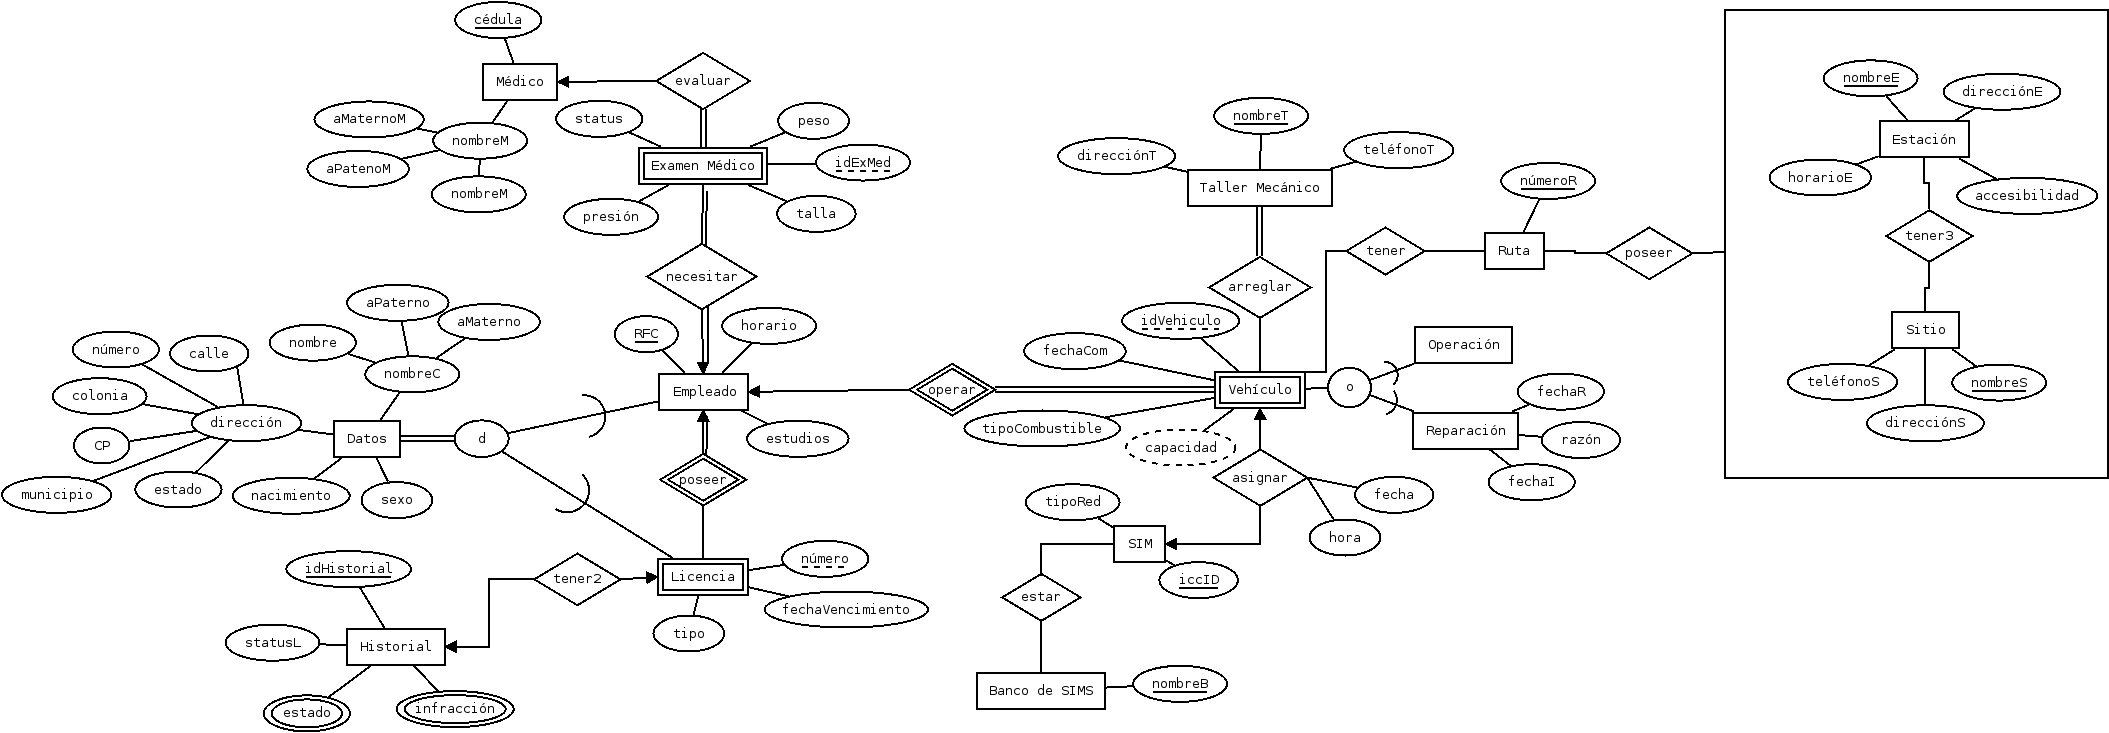
\includegraphics[scale=0.2]{practica5.png}

        Al modelo anterior se le hicieron algunos cambios con respecto al que mostramos en la práctica anterior.
        Los cambios son los siguientes:

        <'\begin{itemize}
            \item Agregamos más atributos a la entidad "Médico".
            \item Corregimos la relación poseer, tener2.
            \item Agregamos un identificador a "Examen Médico" y a "Ruta".
            \item Agregamos atributos a "Historial".
        \end{itemize}

        Para el modelo relacional seguimos lo siguiente:\vspace{.2cm}

        \begin{itemize}
            \item[Lunes -]    Realizamos los cambios al modelo entidad relación para que se adecuara al caso prueba.
            \item[Martes -]   Discutimos sobre las tablas e hicimos un primer borrador del modelo.
            \item[Jueves -]   Acordamos que el modelo tenía una mejoría e realizamos la traducción final al modelo
                            relacional.   
        \end{itemize}

        El modelo relacional se ve a continuación:

            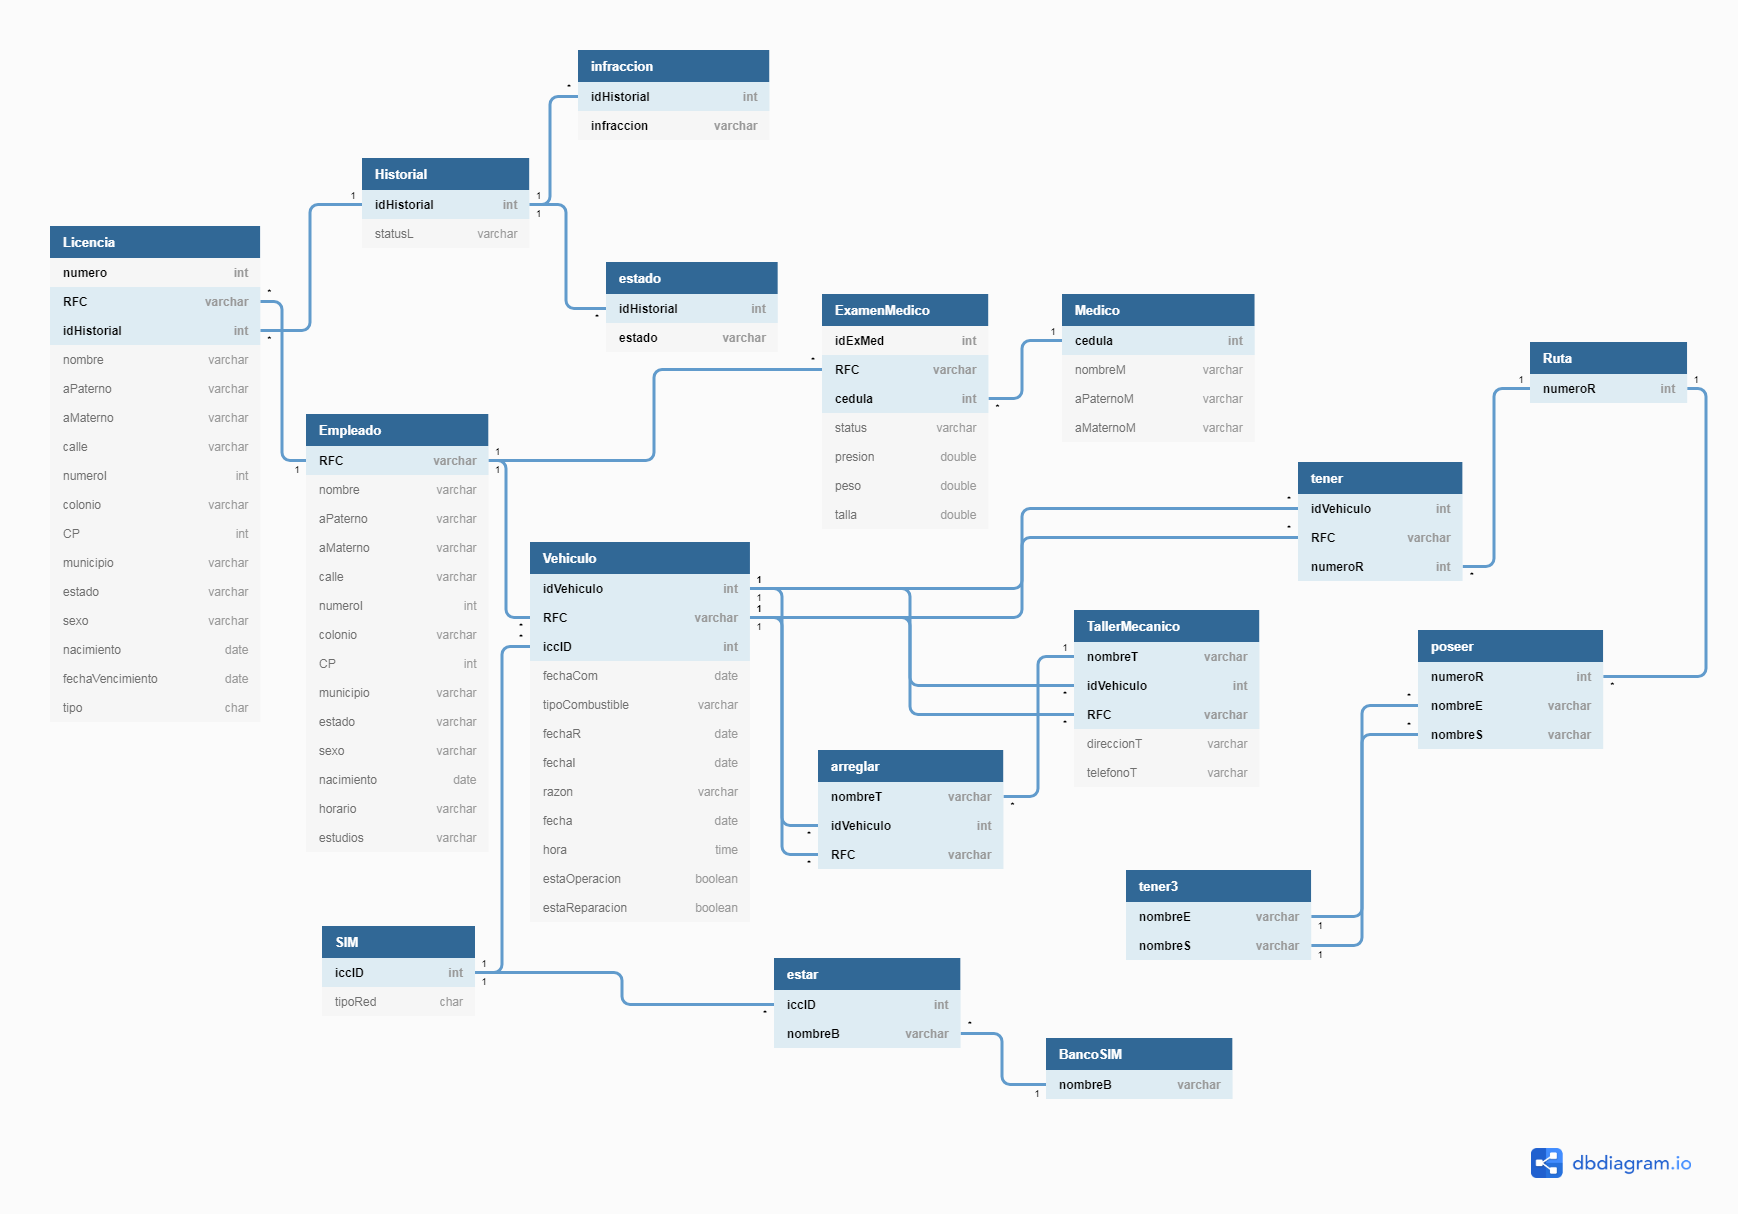
\includegraphics[scale=0.25]{CasPrueba.png}

        \subsection*{SQL}
        En la segunda parte de la práctica creamos una base de datos con el siguiente script:
        
            USE master;\vspace{.3cm}

            PRINT N"Validamos si la base de datos no existe"; \vspace{.1cm}

            IF NOT EXISTS (SELECT 1 FROM sys.databases WHERE [name] = "FbdEjemplo")\vspace{.1cm}

            BEGIN\vspace{.1cm}

            PRINT N"Base no existe"; \vspace{.3cm}

            CREATE DATABASE FbdEjemplo\vspace{.1cm}

            ON PRIMARY\vspace{.1cm}

            (\vspace{.1cm}

                NAME = "FbdEjemplo",\vspace{.1cm}

                FILENAME = "/fbd/fundamentos/FbdEjemplo.mdf ",\vspace{.1cm}

                SIZE = 10MB,\vspace{.1cm}

                MAXSIZE = UNLIMITED,\vspace{.1cm}

                FILEGROWTH = 50\%\vspace{.1cm}
        
            )\vspace{.1cm}

            LOG ON\vspace{.1cm}

            (\vspace{.1cm}

                NAME = "FbdEjemplo_log",\vspace{.1cm}

                FILENAME =  "/fbd/fundamentos/FbdEjemplo_log.ldf",\vspace{.1cm}

                SIZE = 2MB,\vspace{.1cm}

                MAXSIZE = 100MB,\vspace{.1cm}

                FILEGROWTH = 2MB\vspace{.1cm}

            );\vspace{.1cm}

            PRINT N"Base de datos creada correctamente"; \vspace{.1cm}

            END;\vspace{.1cm}

            ELSE\vspace{.1cm}

            PRINT N"Base de datos ya existe";\vspace{.1cm}

            GO\vspace{.1cm}

    \section*{Conclusión}
    Algunos problemas que presentamos en el desarrolo de esta prática fue en la ejecución del script de SQL, pero al
    final entendimos cómo debía ser ejecutado. En el caso del modelo relacional, tuvimos una mejor compresión de cómo
    traducir de una manera cuidadosa y rápida.\vspace{.3cm}
    
    En conclusión, la traducción del modelo entidad-relación al modelo relacional nos hace ver de manera más clara
    las relaciones que existen entre las distintas entidades que éste conformado; y T-SQL es un lenguaje muy útil 
    pero un poco problemático.

\end{document}